% =====================================================================
% ELMED219: Maskinlæring – grunnleggende konsepter (M01-M10)
% Beamer-presentasjon i widescreen (16:9)
% =====================================================================
\documentclass[aspectratio=169, 11pt]{beamer}

% =====================================================================
% PAKKER
% =====================================================================
\usepackage[utf8]{inputenc}
\usepackage[T1]{fontenc}
\usepackage[norsk]{babel}
\usepackage{graphicx}
\usepackage{tikz}
\usetikzlibrary{shapes.geometric, arrows, positioning, shapes.symbols}
\usepackage{booktabs}
\usepackage{amsmath}
\usepackage{fontawesome5}

% =====================================================================
% TEMA OG FARGER
% =====================================================================
\usetheme{Madrid}
\usecolortheme{default}

% UiB-farger
\definecolor{uibblue}{RGB}{0, 61, 115}
\definecolor{uibred}{RGB}{175, 28, 44}
\definecolor{lightgray}{RGB}{245, 245, 245}

\setbeamercolor{palette primary}{bg=uibblue, fg=white}
\setbeamercolor{palette secondary}{bg=uibblue!80, fg=white}
\setbeamercolor{palette tertiary}{bg=uibblue!60, fg=white}
\setbeamercolor{structure}{fg=uibblue}
\setbeamercolor{title}{fg=uibblue}
\setbeamercolor{frametitle}{fg=uibblue, bg=lightgray}
\setbeamercolor{block title}{bg=uibblue, fg=white}
\setbeamercolor{block body}{bg=lightgray}

% Fjern navigasjonssymboler
\setbeamertemplate{navigation symbols}{}

% Slide-nummer
\setbeamertemplate{footline}{
    \hfill\insertframenumber/\inserttotalframenumber\hspace{2mm}\vspace{2mm}
}

% =====================================================================
% TITTELINFO
% =====================================================================
\title[M: Maskinlæring]{Maskinlæring -- Grunnleggende konsepter}
\subtitle{Momentliste M01--M10}
\author{ELMED219 / BMED365}
\institute{Universitetet i Bergen}
\date{Våren 2026}

% =====================================================================
% DOKUMENT
% =====================================================================
\begin{document}

% ---------------------------------------------------------------------
% Tittelslide
% ---------------------------------------------------------------------
\begin{frame}
    \titlepage
\end{frame}

% ---------------------------------------------------------------------
% Oversikt
% ---------------------------------------------------------------------
\begin{frame}{Oversikt}
    \tableofcontents
\end{frame}

% =====================================================================
\section{Hva er maskinlæring?}
% =====================================================================

% ---------------------------------------------------------------------
% M01
% ---------------------------------------------------------------------
\begin{frame}{M01: Definere maskinlæring og skille fra tradisjonell programmering}
    
    \begin{columns}
        \begin{column}{0.48\textwidth}
            \textbf{Tradisjonell programmering:}
            \begin{itemize}
                \item Eksplisitte regler definert av programmerer
                \item \texttt{if-else} logikk
                \item Input + Regler $\rightarrow$ Output
            \end{itemize}
            
            \vspace{3mm}
            \textbf{Maskinlæring:}
            \begin{itemize}
                \item Lærer regler fra data
                \item Mønstergjenkjenning
                \item Input + Output $\rightarrow$ Regler (modell)
            \end{itemize}
        \end{column}
        
        \begin{column}{0.48\textwidth}
            \begin{block}{Definisjon}
                \textit{``A computer program is said to learn from experience E with respect to some task T and some performance measure P, if its performance on T, as measured by P, improves with experience E.''}
                \\ \hfill -- Tom Mitchell, 1997
            \end{block}
        \end{column}
    \end{columns}
    
\end{frame}

% ---------------------------------------------------------------------
% M02
% ---------------------------------------------------------------------
\begin{frame}{M02: Supervised vs. Unsupervised læring}
    
    \begin{columns}
        \begin{column}{0.48\textwidth}
            \textbf{\faCheckCircle\ Supervised (veiledet) læring:}
            \begin{itemize}
                \item Data har \textbf{labels} (fasit)
                \item Modellen lærer å predikere labels
                \item Eksempler: Klassifisering, regresjon
                \item Medisinsk: Diagnostisering fra bilder
            \end{itemize}
        \end{column}
        
        \begin{column}{0.48\textwidth}
            \textbf{\faSearch\ Unsupervised (uveiledet) læring:}
            \begin{itemize}
                \item Data uten labels
                \item Finner skjulte mønstre/strukturer
                \item Eksempler: Klynging (clustering)
                \item Medisinsk: Pasient-subgrupper
            \end{itemize}
        \end{column}
    \end{columns}
    
    \vspace{5mm}
    \begin{center}
        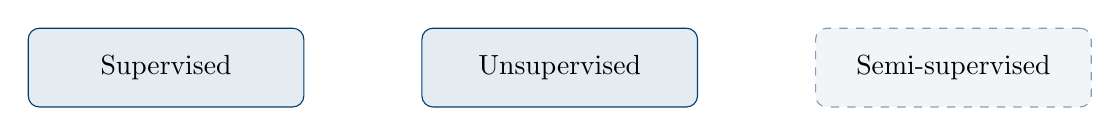
\begin{tikzpicture}
            \node[draw=uibblue, fill=uibblue!10, rounded corners, minimum width=3.5cm, minimum height=1cm] at (0,0) {Supervised};
            \node[draw=uibblue, fill=uibblue!10, rounded corners, minimum width=3.5cm, minimum height=1cm] at (5,0) {Unsupervised};
            \node[draw=uibblue!50, fill=uibblue!5, rounded corners, minimum width=3.5cm, minimum height=1cm, dashed] at (10,0) {Semi-supervised};
        \end{tikzpicture}
    \end{center}
    
\end{frame}

% ---------------------------------------------------------------------
% M03
% ---------------------------------------------------------------------
\begin{frame}{M03: Features (input) og Labels (output)}
    
    \begin{block}{Definisjoner}
        \begin{itemize}
            \item \textbf{Features} ($\mathbf{X}$): Inputvariabler / kjennetegn som beskriver dataene
            \item \textbf{Labels} ($y$): Målvariabel / det vi ønsker å predikere
        \end{itemize}
    \end{block}
    
    \vspace{3mm}
    
    \textbf{Eksempel -- Hjertesykdomsprediksjon:}
    
    \begin{table}
        \centering
        \begin{tabular}{cccc|c}
            \toprule
            \textbf{Alder} & \textbf{Kolesterol} & \textbf{Blodtrykk} & \textbf{BMI} & \textbf{Sykdom?} \\
            \midrule
            55 & 240 & 140 & 28 & Ja \\
            32 & 180 & 120 & 23 & Nei \\
            67 & 210 & 155 & 31 & Ja \\
            \bottomrule
        \end{tabular}
    \end{table}
    
    \begin{center}
        \textcolor{uibblue}{\textbf{Features} $\mathbf{X}$} \hspace{2cm} \textcolor{uibred}{\textbf{Label} $y$}
    \end{center}
    
\end{frame}

% ---------------------------------------------------------------------
% M04
% ---------------------------------------------------------------------
\begin{frame}{M04: Hvorfor trenings- og testsett?}
    
    \textbf{Problemet:} Hvordan vet vi om modellen generaliserer til nye data?
    
    \vspace{3mm}
    
    \begin{columns}
        \begin{column}{0.55\textwidth}
            \begin{block}{Løsningen: Data-splitting}
                \begin{enumerate}
                    \item Del datasettet i to (eller tre) deler
                    \item \textbf{Treningssett} ($\sim$70--80\%): Tren modellen
                    \item \textbf{Testsett} ($\sim$20--30\%): Evaluer på usett data
                    \item (Valideringssett: Tuning av hyperparametre)
                \end{enumerate}
            \end{block}
        \end{column}
        
        \begin{column}{0.4\textwidth}
            
\begin{tikzpicture}[scale=0.8]
                \fill[uibblue!60] (0,0) rectangle (4,1);
                \fill[uibred!60] (4,0) rectangle (5.5,1);
                \node[white] at (2, 0.5) {\small Trening (70\%)};
                \node[white] at (4.75, 0.5) {\small Test};
            \end{tikzpicture}
        \end{column}
    \end{columns}
    
    \vspace{5mm}
    
    \begin{alertblock}{Viktig}
        Modellen skal \textbf{aldri} se testdataene under trening! \\
        Dette simulerer ``real-world'' prediksjoner.
    \end{alertblock}
    
\end{frame}

% ---------------------------------------------------------------------
% M05
% ---------------------------------------------------------------------
\begin{frame}{M05: Overfitting og Underfitting}
    
    \begin{columns}
        \begin{column}{0.32\textwidth}
            \textbf{Underfitting:}
            \begin{itemize}
                \item For enkel modell
                \item Høy bias
                \item Dårlig på både trening og test
            \end{itemize}
            \begin{center}
                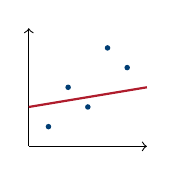
\begin{tikzpicture}[scale=0.5]
                    \draw[->] (0,0) -- (3,0);
                    \draw[->] (0,0) -- (0,3);
                    \fill[uibblue] (0.5,0.5) circle (2pt);
                    \fill[uibblue] (1,1.5) circle (2pt);
                    \fill[uibblue] (1.5,1) circle (2pt);
                    \fill[uibblue] (2,2.5) circle (2pt);
                    \fill[uibblue] (2.5,2) circle (2pt);
                    \draw[uibred, thick] (0,1) -- (3,1.5);
                \end{tikzpicture}
            \end{center}
        \end{column}
        
        \begin{column}{0.32\textwidth}
            \textbf{God tilpasning:}
            \begin{itemize}
                \item Riktig kompleksitet
                \item Balanse
                \item Generaliserer godt
            \end{itemize}
            \begin{center}
                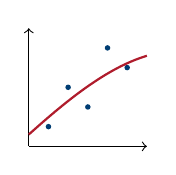
\begin{tikzpicture}[scale=0.5]
                    \draw[->] (0,0) -- (3,0);
                    \draw[->] (0,0) -- (0,3);
                    \fill[uibblue] (0.5,0.5) circle (2pt);
                    \fill[uibblue] (1,1.5) circle (2pt);
                    \fill[uibblue] (1.5,1) circle (2pt);
                    \fill[uibblue] (2,2.5) circle (2pt);
                    \fill[uibblue] (2.5,2) circle (2pt);
                    \draw[uibred, thick] (0,0.3) .. controls (1,1.2) and (2,2) .. (3,2.3);
                \end{tikzpicture}
            \end{center}
        \end{column}
        
        \begin{column}{0.32\textwidth}
            \textbf{Overfitting:}
            \begin{itemize}
                \item For kompleks modell
                \item Høy varians
                \item Lærer støy i dataene
            \end{itemize}
            \begin{center}
                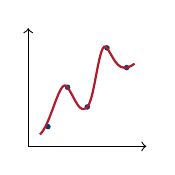
\begin{tikzpicture}[scale=0.5]
                    \draw[->] (0,0) -- (3,0);
                    \draw[->] (0,0) -- (0,3);
                    \fill[uibblue] (0.5,0.5) circle (2pt);
                    \fill[uibblue] (1,1.5) circle (2pt);
                    \fill[uibblue] (1.5,1) circle (2pt);
                    \fill[uibblue] (2,2.5) circle (2pt);
                    \fill[uibblue] (2.5,2) circle (2pt);
                    \draw[uibred, thick] (0.3,0.3) .. controls (0.6,0.6) and (0.8,1.8) .. (1,1.5) .. controls (1.2,1.2) and (1.3,0.8) .. (1.5,1) .. controls (1.7,1.2) and (1.8,2.8) .. (2,2.5) .. controls (2.2,2.2) and (2.3,1.8) .. (2.7,2.1);
                \end{tikzpicture}
            \end{center}
        \end{column}
    \end{columns}
    
    \vspace{5mm}
    
    \begin{block}{Kjennetegn på overfitting}
        Stor forskjell mellom trenings-ytelse og test-ytelse
    \end{block}
    
\end{frame}

% ---------------------------------------------------------------------
% M06
% ---------------------------------------------------------------------
\begin{frame}{M06: Bias-Variance Trade-off}
    
    \textbf{Totalt prediksjonsfeil = Bias² + Varians + Irreducible Error}
    
    \vspace{3mm}
    
    \begin{columns}
        \begin{column}{0.48\textwidth}
            \textbf{Bias (systematisk feil):}
            \begin{itemize}
                \item Feil pga. forenklet modell
                \item Høy bias $\rightarrow$ underfitting
                \item Modellen ``misser'' mønsteret
            \end{itemize}
            
            \vspace{3mm}
            
            \textbf{Varians (tilfeldig feil):}
            \begin{itemize}
                \item Sensitiv for små endringer i data
                \item Høy varians $\rightarrow$ overfitting
                \item Modellen ``husker'' støy
            \end{itemize}
        \end{column}
        
        \begin{column}{0.48\textwidth}
            \begin{center}
                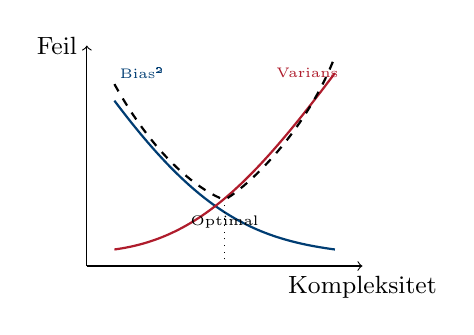
\begin{tikzpicture}[scale=0.7]
                    \draw[->] (0,0) -- (5,0) node[below] {\small Kompleksitet};
                    \draw[->] (0,0) -- (0,4) node[left] {\small Feil};
                    
                    \draw[uibblue, thick] (0.5,3) .. controls (2,1) and (3,0.5) .. (4.5,0.3);
                    \draw[uibred, thick] (0.5,0.3) .. controls (2,0.5) and (3,1.5) .. (4.5,3.5);
                    \draw[black, thick, dashed] (0.5,3.3) .. controls (1.5,1.5) and (2.5,1.2) .. (2.5,1.2) .. controls (3,1.5) and (4,2.5) .. (4.5,3.8);
                    
                    \node[uibblue] at (1, 3.5) {\tiny Bias²};
                    \node[uibred] at (4, 3.5) {\tiny Varians};
                    \node at (2.5, 0.8) {\tiny Optimal};
                    
                    \draw[dotted] (2.5, 0) -- (2.5, 1.2);
                \end{tikzpicture}
            \end{center}
        \end{column}
    \end{columns}
    
    \vspace{3mm}
    
    \begin{block}{Målet}
        Finn balansen som minimerer \textbf{total feil} på nye data
    \end{block}
    
\end{frame}

% =====================================================================
\section{Validering og modelltyper}
% =====================================================================

% ---------------------------------------------------------------------
% M07
% ---------------------------------------------------------------------
\begin{frame}{M07: K-fold kryssvalidering}
    
    \textbf{Problem:} Ett enkelt train/test-split kan gi tilfeldige resultater
    
    \vspace{3mm}
    
    \textbf{Løsning: K-fold Cross-Validation}
    \begin{enumerate}
        \item Del data i $k$ like store deler (``folds'')
        \item For hver fold: bruk den som test, resten som trening
        \item Gjennomsnitt av alle $k$ evalueringer
    \end{enumerate}
    
    \vspace{3mm}
    
    \begin{center}
        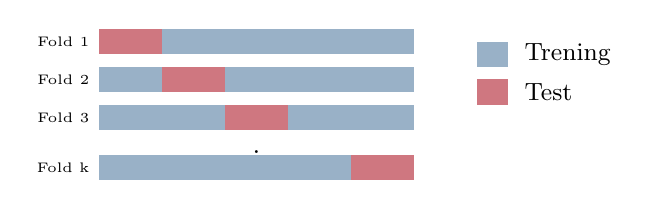
\begin{tikzpicture}[scale=0.8]
            % Fold 1
            \fill[uibred!60] (0,2) rectangle (1,2.4);
            \fill[uibblue!40] (1,2) rectangle (5,2.4);
            \node[left] at (0, 2.2) {\tiny Fold 1};
            
            % Fold 2
            \fill[uibblue!40] (0,1.4) rectangle (1,1.8);
            \fill[uibred!60] (1,1.4) rectangle (2,1.8);
            \fill[uibblue!40] (2,1.4) rectangle (5,1.8);
            \node[left] at (0, 1.6) {\tiny Fold 2};
            
            % Fold 3
            \fill[uibblue!40] (0,0.8) rectangle (2,1.2);
            \fill[uibred!60] (2,0.8) rectangle (3,1.2);
            \fill[uibblue!40] (3,0.8) rectangle (5,1.2);
            \node[left] at (0, 1) {\tiny Fold 3};
            
            % etc
            \node at (2.5, 0.4) {$\vdots$};
            
            \fill[uibblue!40] (0,0) rectangle (4,0.4);
            \fill[uibred!60] (4,0) rectangle (5,0.4);
            \node[left] at (0, 0.2) {\tiny Fold k};
            
            % Legend
            \fill[uibblue!40] (6, 1.8) rectangle (6.5, 2.2);
            \node[right] at (6.6, 2) {\small Trening};
            \fill[uibred!60] (6, 1.2) rectangle (6.5, 1.6);
            \node[right] at (6.6, 1.4) {\small Test};
        \end{tikzpicture}
    \end{center}
    
    \vspace{3mm}
    
    \textbf{Fordeler:} Mer robust estimat, bruker all data for både trening og testing
    
\end{frame}

% ---------------------------------------------------------------------
% M08
% ---------------------------------------------------------------------
\begin{frame}{M08: Baseline-modell}
    
    \begin{block}{Hva er en baseline?}
        En \textbf{enkel referansemodell} som vår ML-modell må slå for å være nyttig.
    \end{block}
    
    \vspace{3mm}
    
    \textbf{Eksempler på baselines:}
    
    \begin{itemize}
        \item \textbf{Klassifisering:} Prediker alltid majoritetsklassen
        \begin{itemize}
            \item Datasett med 90\% friske, 10\% syke $\rightarrow$ baseline accuracy = 90\%
        \end{itemize}
        \item \textbf{Regresjon:} Prediker alltid gjennomsnittsverdien
        \item \textbf{Tidsserie:} Bruk forrige verdi som prediksjon
    \end{itemize}
    
    \vspace{5mm}
    
    \begin{alertblock}{Hvorfor viktig?}
        \begin{itemize}
            \item 90\% accuracy høres imponerende ut, men ikke hvis baseline er 90\%
            \item Viser om ML tilfører \textbf{faktisk verdi}
            \item Avslører ubalanserte datasett
        \end{itemize}
    \end{alertblock}
    
\end{frame}

% ---------------------------------------------------------------------
% M09
% ---------------------------------------------------------------------
\begin{frame}{M09: Klassifisering vs. Regresjon}
    
    \begin{columns}
        \begin{column}{0.48\textwidth}
            \textbf{\faThLarge\ Klassifisering:}
            \begin{itemize}
                \item Predikerer \textbf{kategorier/klasser}
                \item Diskrete utfall
                \item Eksempler:
                \begin{itemize}
                    \item Syk / Frisk
                    \item Kreft type A / B / C
                    \item Lesjonsklassifikasjon
                \end{itemize}
            \end{itemize}
            
            \vspace{3mm}
            
            \textbf{Evalueringsmetrikker:}
            \begin{itemize}
                \item Accuracy, Precision, Recall
                \item F1-score, AUC-ROC
            \end{itemize}
        \end{column}
        
        \begin{column}{0.48\textwidth}
            \textbf{\faChartLine\ Regresjon:}
            \begin{itemize}
                \item Predikerer \textbf{kontinuerlige verdier}
                \item Numeriske utfall
                \item Eksempler:
                \begin{itemize}
                    \item Blodtrykk
                    \item Forventet levetid
                    \item Medikamentdosering
                \end{itemize}
            \end{itemize}
            
            \vspace{3mm}
            
            \textbf{Evalueringsmetrikker:}
            \begin{itemize}
                \item MSE, RMSE, MAE
                \item R² (forklart varians)
            \end{itemize}
        \end{column}
    \end{columns}
    
\end{frame}

% ---------------------------------------------------------------------
% M10
% ---------------------------------------------------------------------
\begin{frame}{M10: Enkle ML-modeller}
    
    \begin{columns}
        \begin{column}{0.32\textwidth}
            \textbf{Beslutningstre:}
            \begin{itemize}
                \item Serier av ja/nei-spørsmål
                \item Lett å tolke
                \item Kan overfitte
            \end{itemize}
            \begin{center}
                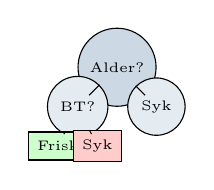
\begin{tikzpicture}[scale=0.5, every node/.style={font=\tiny}]
                    \node[draw, circle, fill=uibblue!20] (root) at (1.5,2) {Alder?};
                    \node[draw, circle, fill=uibblue!10] (l) at (0.5,1) {BT?};
                    \node[draw, circle, fill=uibblue!10] (r) at (2.5,1) {Syk};
                    \node[draw, rectangle, fill=green!20] (ll) at (0,0) {Frisk};
                    \node[draw, rectangle, fill=red!20] (lr) at (1,0) {Syk};
                    \draw (root) -- (l);
                    \draw (root) -- (r);
                    \draw (l) -- (ll);
                    \draw (l) -- (lr);
                \end{tikzpicture}
            \end{center}
        \end{column}
        
        \begin{column}{0.32\textwidth}
            \textbf{k-Nearest Neighbors:}
            \begin{itemize}
                \item Finn $k$ mest like eksempler
                \item Majoritetsvotering
                \item Enkel, men treg
            \end{itemize}
            \begin{center}
                
\begin{tikzpicture}[scale=0.5]
                    \fill[uibblue] (0.5,0.5) circle (3pt);
                    \fill[uibblue] (0.8,1) circle (3pt);
                    \fill[uibblue] (1,0.7) circle (3pt);
                    \fill[uibred] (2,2) circle (3pt);
                    \fill[uibred] (2.3,1.8) circle (3pt);
                    \fill[uibred] (1.8,2.2) circle (3pt);
                    \node[draw, star, fill=green!50, scale=0.5] at (1.5,1.3) {};
                    \draw[dashed] (1.5,1.3) circle (0.6);
                \end{tikzpicture}
            \end{center}
        \end{column}
        
        \begin{column}{0.32\textwidth}
            \textbf{Logistisk regresjon:}
            \begin{itemize}
                \item Lineær grense
                \item Gir sannsynligheter
                \item Rask og tolkbar
            \end{itemize}
            \begin{center}
                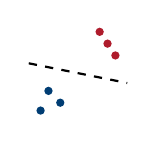
\begin{tikzpicture}[scale=0.5]
                    \fill[uibblue] (0.3,0.3) circle (3pt);
                    \fill[uibblue] (0.5,0.8) circle (3pt);
                    \fill[uibblue] (0.8,0.5) circle (3pt);
                    \fill[uibred] (2,2) circle (3pt);
                    \fill[uibred] (2.2,1.7) circle (3pt);
                    \fill[uibred] (1.8,2.3) circle (3pt);
                    \draw[thick, dashed] (0,1.5) -- (2.5,1);
                \end{tikzpicture}
            \end{center}
        \end{column}
    \end{columns}
    
    \vspace{5mm}
    
    \begin{block}{Tips}
        Start alltid med enkle modeller før du prøver komplekse!
    \end{block}
    
\end{frame}

% ---------------------------------------------------------------------
% Oppsummering
% ---------------------------------------------------------------------
\begin{frame}{Oppsummering: M01--M10}
    
    \begin{columns}
        \begin{column}{0.48\textwidth}
            \textbf{Nøkkelkonsepter:}
            \begin{itemize}
                \item ML lærer fra data (ikke eksplisitte regler)
                \item Supervised vs. Unsupervised
                \item Features (X) og Labels (y)
                \item Train/Test split
                \item Overfitting vs. Underfitting
            \end{itemize}
        \end{column}
        
        \begin{column}{0.48\textwidth}
            \textbf{Beste praksis:}
            \begin{itemize}
                \item Bruk kryssvalidering
                \item Sammenlign med baseline
                \item Klassifisering $\neq$ Regresjon
                \item Start enkelt (beslutningstre, k-NN)
                \item Balanse mellom bias og varians
            \end{itemize}
        \end{column}
    \end{columns}
    
    \vspace{5mm}
    
    \begin{block}{Medisinsk relevans}
        ML-modeller brukes i dag til:
        \begin{itemize}
            \item Diagnostisk støtte (bildediagnostikk, patologi)
            \item Risikoprediksjon (hjertesykdom, kreft)
            \item Pasientstratifisering (persontilpasset medisin)
        \end{itemize}
    \end{block}
    
\end{frame}

\end{document}
